% Based on the answer by qubyte at 
% http://tex.stackexchange.com/questions/9767/whats-a-good-package-for-typesetting-quantum-circuits
\documentclass[12pt]{standalone}
\usepackage{tikz}

\usetikzlibrary{backgrounds,calc,decorations.pathreplacing}
% Dirac Kets
\newcommand{\ket}[1]{\ensuremath{\left|#1\right\rangle}}

\begin{document}
    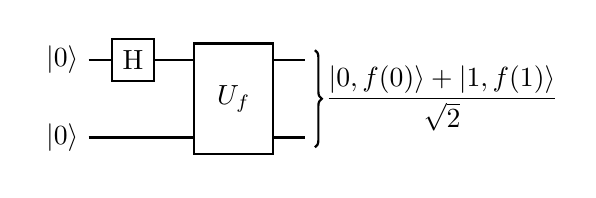
\begin{tikzpicture}[thick,cross/.style={path picture={ 
  \draw[black]
(path picture bounding box.south) -- (path picture bounding box.north);
}}]

    % `operator' will only be used by most gates.
    % `cnot' will refer to CNOT gates.
    % `phase' is used for controlled gates.
    \tikzstyle{operator} = [draw,fill=white,minimum size=1.5em]
    \tikzstyle{cnot} = [draw,cross,circle,minimum size=5pt]
    \tikzstyle{phase} = [draw,fill,shape=circle,minimum size=5pt,inner sep=0pt]
    %
    \matrix[row sep=0.4cm, column sep=0.8cm] (circuit) {

    % First row.
    \node (q1) {\ket{0}}; 
    \coordinate (start1); &[-0.5cm] 
    \node[operator] (O11) {H}; &
    &
    &[-0.5cm] 
    \coordinate (end1);\\

    \node (q2) {\ket{0}}; 
    \coordinate (start2); &[-0.5cm] 
    &
    &
    &[-0.5cm] 
    \coordinate (end2);\\
    };
    \draw [thick,black,fill=white] (0.3,-2em) rectangle (1.3,2em);
    \node at (0.8,0) (Uf) {$U_f$};
    
    
    \draw[decorate,decoration={brace},thick]
        ($(circuit.north east)-(0cm,0.3cm)$)
        to node[midway,right] (bracket) {$\displaystyle\frac{\ket{0,f(0)}+\ket{1,f(1)}}{\sqrt{2}}$}
        ($(circuit.south east)+(0cm,0.3cm)$);
    \begin{pgfonlayer}{background}
        % Draw lines.
        \draw[thick] (q1) -- (end1) (q2) -- (end2);
    \end{pgfonlayer}
    %
    \end{tikzpicture}
\end{document}
